\documentclass[letter]{article}

%% Language and font encodings
\usepackage[spanish]{babel}
\usepackage{fontspec}
\usepackage{float} 

%% Sets page size and margins
\usepackage[letterpaper,top=2cm,bottom=2cm,left=2.5cm,right=2.5cm]{geometry}

%% Useful packages
\usepackage{amsmath,amsthm,amssymb,amsfonts}
\usepackage{graphicx}
\usepackage[colorinlistoftodos]{todonotes}
\usepackage[colorlinks=true, allcolors=blue]{hyperref}

\title{Reporte de simulación del experimento X}

\author{Nombre: xxxxx \\
        Nombre: yyyyy \\
}
%\date{dd/mm/yyyy}

\begin{document}
\renewcommand{\tablename}{Tabla} 
\maketitle

\section{Respuestas al cuestionario previo}

\begin{enumerate}

    \item Respuesta a la pregunta 1. \textbf{Texto en Negrita}.
    
    \item Respuesta a la pregunta 2. \textit{Texto en Cursiva}.
    
\end{enumerate}

\section{Resultados de la simulación}

Se midió la corriente y la tensión indicados en el inciso 4 del procedimiento se muestran en la tabla \ref{tab:medicion_I_V}.

\begin{table} [ht]
    \centering
    \caption{Título de la tabla}
    \label{tab:medicion_I_V}
    \begin{tabular}{|c|c|c|}
        \hline 
        Medición & Corriente (mA) & Tensión (V) \\ 
        \hline 
        1  & 3,45 & 5,00 \\ 
        \hline 
        2 & 4,65 & 7,32 \\ 
        \hline 
    \end{tabular} 
\end{table}

En la figura \ref{fig:graf} se observa un plano cartesiano.

\begin{figure}[htb]
    \centering
    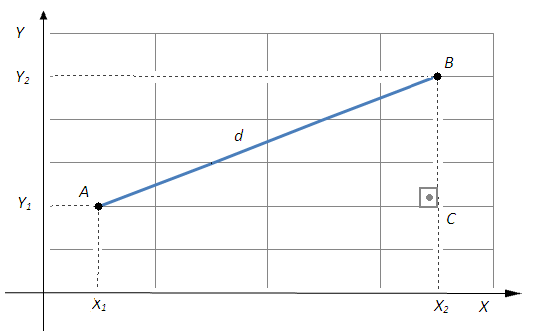
\includegraphics[width=0.5\textwidth]{Plano_cartesiano.png}
    \caption{Gráfica de ejemplo}
    \label{fig:graf}
\end{figure} 

La tabla \ref{tab:datos_equipos} contiene los datos obtenidos del equipo.

\begin{table}
    \centering
    \caption{Título de la tabla}
    \label{tab:datos_equipos}
    \begin{tabular}{|c|c|}
        \hline
        Dato & Valor\\
        \hline
        Identificación & Dato \\
        Resolución en dígitos & Dato \\
        Resolución en escala de 200 mV & Dato \\
        Resolución en escala de 2 V & Dato \\
        Resolución en escala de 20 V & Dato \\
        Resolución en escala de 200 V & Dato \\
        Resolución en escala de 2000 V & Dato \\
        Resolución en escala de 20 mA & Dato \\
        Resolución en escala de 200 mA & Dato \\
        Resolución en escala de 2 A & Dato \\
        Resolución en escala de 20 A & Dato \\
        Resolución en escala de 200 \(\Omega\) & Dato \\
        Resolución en escala de 2 k\(\Omega\) & Dato \\
        Resolución en escala de 20 k\(\Omega\) & Dato \\
        Resolución en escala de 200 k\(\Omega\) & Dato \\
        Resolución en escala de 2 M\(\Omega\) & Dato \\
        Resolución en escala de 20 M\(\Omega\) & Dato \\
        Resolución en escala de 200 M\(\Omega\) & Dato \\
        Error de cero en modo ohmímetro & Dato \\
        Error de cero en modo voltímetro & Dato \\
        Error de cero en modo amperímetro & Dato \\
        Sensibilidad del instrumento como voltímetro & Dato \\
        Sensibilidad del instrumento como amperímetro & Dato \\
        Sensibilidad del instrumento como ohmímetro & Dato \\
        Valor máximo de tensión que puede medir & Dato \\
        Valor máximo de corriente que puede medir & Dato \\
        Valor máximo de resistencia que puede medir & Dato \\
        \hline 
    \end{tabular} 
\end{table}

\section{Reflexiones finales}

\begin{enumerate}

    \item Respuesta a la pregunta 1.
    
    \item Respuesta a la pregunta 2.

\end{enumerate}

\section{Adicional}

Ejemplos de ecuaciones:
\begin{itemize}

    \item Ecuación en el renglón $A=\cfrac{b}{c}$, $y = \int_{x=0}^{x=2 \pi + 10} f(x) \cdot dx$ y $ \sqrt{(a_1-b_1)^2 + (a_2-b_2)^2} $
    
    \item Centradas en la página:
    
    $$A=\cfrac{b}{c}$$
    $$y = \int_{x=0}^{x=2 \pi + 10} f(x) \cdot dx$$
    $$ \sqrt{(a_1-b_1)^2 + (a_2-b_2)^2} $$

\end{itemize}

%expor aqui as conclusões que retiraram do trabalho

\end{document}